%%\documentstyle[twocolumn,jsaiac]{article}
%%\documentstyle[twocolumn,jsaiac]{article}
\documentclass[a4paper,twocolumn]{article}
%\documentclass[dvipdfmx,a4paper,twocolumn]{article}


\usepackage{jsaiac}

\usepackage{amsthm}
\usepackage{amsfonts}
\usepackage{amsmath}
\usepackage{amssymb,bbm}
\usepackage{dsfont}
\usepackage{bm}
\usepackage{graphicx}
\usepackage{algorithm}
\usepackage{algorithmic}

\usepackage{color}

\newcommand{\R}{\mathbb{R}}
\newcommand{\one}{\mathds{1}}
\newcommand{\mat}[1]{\mathbf{#1}}
%\renewcommand{\vec}[1]{\mathbf{#1}}
\renewcommand{\vec}[1]{\bm{#1}}

\newcommand{\changeHK}[1]{\textcolor{black}{#1}}

\newcommand{\changeSX}[1]{\textcolor{black}{#1}}

%%Title:
\title{An Inexact Penalty Method for Fast Unbalanced \protect\\ Optimal Transport Optimization}

%%Contact address:
\address{Waseda University, 3-4-1 Okubo, Shinjuku-ku, Tokyo 169-8555, Japan. Email: $<$suxun$\_$opt@asagi.waseda.jp$>$}

%%Name of authors:
\author{%
Xun Su\first
\and
Hiroyuki Kasai\second
}

%%Affiliations:
\affiliate{
\first{} WASEDA University, Department of Communications and Computer Engineering, Graduate \protect\\School of Fundamental Science and Engineering\\
\second{} WASEDA University, Department of Communications and Computer Engineering, School of \protect\\ Fundamental Science and Engineering
}

%%
%\Vol{28} %% <-- 25
%\session{0A0-00}%% <-- ID

\begin{abstract}
With the increasing application of Optimal Transport (OT) in machine learning, the unbalanced optimal transport (UOT) problem, as a variant of optimal transport, has gained attention for its improved generality. There is an urgent need for fast algorithms that can efficiently handle large penalty parameters. In this paper, we propose to use the Inexact penalty to make the Majorize-Minimization algorithm converge quickly even in UOT with large penalties. By using a dynamic scheme, we can successfully compute better and sparser solutions for the large penalty parameter and approach the computational speed of the well-known Sinkhorn algorithm, which sacrifices accuracy by adding an entropy item.
\end{abstract}

%\setcounter{page}{1}
\def\Style{``jsaiac.sty''}
\def\BibTeX{{\rm B\kern-.05em{\sc i\kern-.025em b}\kern-.08em%
T\kern-.1667em\lower.7ex\hbox{E}\kern-.125emX}}
\def\JBibTeX{\leavevmode\lower .6ex\hbox{J}\kern-0.15em\BibTeX}
\def\LaTeXe{\LaTeX\kern.15em2$_{\textstyle\varepsilon}$}

\begin{document}
\maketitle

\section{Introduction}
\label{sec:int}

Optimal transport (OT) has gained popularity in the fields of machine learning and statistical learning due to its ability to measure the distance between two probability measures. New methods that combine OT have outperformed traditional methods in areas such as domain adaptation \cite{Courty_PAMI_2017} and generative models \cite{arjovsky2017wasserstein}. Recently, OT theory has been applied to various technical fields such as graph analysis \cite{Huang_SigPro_2020,Huang_ICASSP_2021,Fang_AAAI_2023} and sequential data analysis \cite{Horie_EUSIPCO_2022}. The rise in popularity of OT is largely due to the introduction of Sinkhorn's algorithm \cite{Cuturi_NIPS_2013} for the entropy-regularized Kantorovich formulation problem, which has reduced the computational burden associated with large-scale problems. Despite its success, the standard OT problem has a limitation in that it only handles {\it balanced} samples. To accommodate a wider range of applications with {\it unbalanced} samples, some relaxed OT has been proposed, which include the partial OT (POT) \cite{ferradans2013regularized}, the semi-relaxed OT (SROT) \cite{fukunaga_icassp2022,fukunaga_srsinkhorn}, and the unbalanced optimal transport (UOT) \cite{Caffarelli_AM_2010,chizat2017scaling}. The UOT has been proposed. UOT replaces the equality constraints with a KL divergence as a penalty function, and it is solvable by adding an entropic regularization term and using Sinkhorn's algorithm. Although it is fast, scalable, and differentiable, it suffers from instability, and larger errors in solution compared to other regularizers.

Recently, Chapel et al. proposed a Majorization-Maximization algorithm to solve the UOT problem without adding an entropy part by considering the mutual connection between the UOT problem and the non-negative matrix factorization problem \cite{Chapel_NeurIPS_2021}. The algorithm is computable in GPU form, similar to Sinkhorn's algorithm, but it is still slower, especially for large penalization terms. In this paper, we propose to combine the inexact penalty method, which was first introduced by \cite{pmlr-v115-xie20b} in the OT community and has been adapted in Augmented Lagrangian methods for many years, with the MM algorithm, to speed up the optimization process. Our method is simple and effective, and can greatly improve the computational speed of the MM algorithm with larger penalization terms.

\section{Preliminaries}
%\subsection{Preliminaries}
We use $\| \cdot \|_2$ to represent the Euclidean norm. $\mathbb{R}^n$ denotes $n$-dimensional Euclidean space, and $\mathbb{R}^n_+$ denotes the set of vectors in which all elements are non-negative. $\mathbb{R}^{n \times m}_+$ stands for the set of $n \times m$ matrices in which all elements are non-negative. We present vectors as bold lower-case letters $\vec{a},\vec{b},\vec{c},\dots$ and matrices as bold-face upper-case letters $\mat{A},\mat{B},\mat{C},\dots$. The $i$-th element of $\vec{a}$ and the element at the $(i,j)$ position of $\mat{A}$ are stated respectively as $a_i$ and ${A}_{i,j}$. In addition, $\one_n \in \mathbb{R}^n$ is the $n$-dimensional vector in which all elements are one.
%For $\vec{x}$ and $\vec{y}$ of the same size, $\langle \vec{x},\vec{y} \rangle = \vec{x}^T\vec{y}$ is the Euclidean dot-product between vectors.
For two matrices of the same size $\mat{A}$ and $\mat{B}$, $\langle \mat{A},\mat{B}\rangle={\rm tr}(\mat{A}^T\mat{B})$ is the Frobenius dot-product. 

%\subsection{Backgrounds}
The balanced OT problem is defined as
\begin{eqnarray}
\label{Eq:Standard_OT}
\operatorname{OT}(\vec{a},\vec{b}) &:=& \min_{ \mat{T} \in \R_{+}^{n \times m}} \langle \mat{C}, \mat{T} \rangle \\
\text{subject\ to}&& \mat{T} \one_n= \vec{a}, \mat{T}^{T}\one_m = \vec{b}. \notag
\end{eqnarray}
Then, by adding the KL divergence to penalize the difference, the UOT problem is defined as:
\begin{align}
\label{eq:uot}
&\operatorname{UOT}(\vec{a},\vec{b}) := \notag\\
&\min_{\mat{T} \in \R_{+}^{n \times m}} \langle \mat{C}, \mat{T} \rangle+ \tau KL(\mat{T} \one_n,\vec{a}) + \tau KL(\mat{T}^{T} \one_n,\vec{b}),
\end{align}
where $\mathrm{KL}(\vec{x},\vec{y})$ stands for the KL divergence between $\vec{x} \in \mathbb{R}_+^n$ and $\vec{y} \in \mathbb{R}_+^n$, which is defined as $\sum_i \vec{x}_i \log {(\vec{x}_i/\vec{y}_i)} - \vec{x}_i + \vec{y}_i$. For this UOT problem, Chapel et al. consider it as a composite optimization problem \cite{Chapel_NeurIPS_2021}, where they propose the MM algorithm to solve the UOT problem:

\begin{align}
\label{eq:update}
&\mat{T}^{(k+1)}=\notag\\
&\operatorname{diag}\left(\frac{\vec a}{\mat{T}^{(k)} \one_m}\right)^{\frac{1}{2}}\left(\mat{T}^{(k)} \odot \exp \left(-\frac{\mat C}{2 \lambda}\right)\right)
\operatorname{diag}\left(\frac{\vec{b}}{\mat{T}^{(k) \top} \one_n}\right)^{\frac{1}{2}},\notag\\
\end{align}

It is worth noting that the updating formula presented in Eq.~(\ref{eq:update}) bears remarkable similarities with the widely popular Sinkhorn's algorithm, as it relies solely on matrix multiplication. While Sinkhorn's algorithm solves Eq.~(\ref{eq:uot}) with an additional regularization term $\epsilon \mat H(\mat T) = \epsilon \langle \mat T,\ln(\mat T - 1)\rangle$ using an alternative matrix multiplication method, it shares a similar computational structure with MM algorithm. This feature also allows for the use of GPU acceleration to speed up the computation process.


\section{Inexact Penalized MM algorithm}
However, we observed that the MM algorithm suffers from performance degradation for larger $\tau$ values, as illustrated in Figure~\ref{Fig:ex2}. Similarly, the Augmented Lagrangian Method (ALM) also uses an additional quadratic penalization term to expedite convergence but is plagued by an ill-conditioned Hessian matrix \cite{doi:10.1137/1.9781611973365}.
To overcome these limitations, we introduce a novel Inexact Penalized MM algorithm (MM-IP) that incorporates a {\it dynamic penalization term}, gradually increasing its influence throughout the optimization process. This approach has been previously employed in ALM research, and we demonstrate its effectiveness in our proposed algorithm. Our proposed algorithm is summarized in {\bf Algorithm.~\ref{Alg1}}, where we set a small constant $q \in \R_+ $ and gradually increase the value of $\tilde{\tau}\in \R_+$ as the optimization error reduces. This inexact optimization process enables our algorithm to obtain a sparser initialization, allowing it to avoid the ill-conditioned Hessian matrix issue encountered in the early stages of optimization.

\begin{algorithm}[t]
\caption{Inexact Penalty Method UOT}
\begin{algorithmic}[t]
\label{Alg1}
\renewcommand{\algorithmicrequire}{\textbf{Input:}}
\renewcommand{\algorithmicensure}{\textbf{Output:}}
\REQUIRE $\mat{T}^0, \mat C, \tilde{\tau}, \tau, q$
\ENSURE $\mat T^{K}$
\STATE $\mat G = \operatorname{exp}(-\frac{\mat{C}}{2\tilde{\tau}})$
\FOR {$k = 1 \text{ to } K$}

\STATE $\vec{u} = (\frac{\vec{a}}{\mat T \one_n})^{\frac{1}{2}}, \vec v=(\frac{\vec{b}}{\mat{T}^{T} \one_m})^{\frac{1}{2}}$
\STATE $\mat{T}^{k} = \mat T^{k} \odot ( \vec{u}^{T} \mat G \vec{v})$
\STATE $err = \|\mat T^{k-1} - \mat T^{k}\|_2$
\IF {$err \leq \frac{q}{\tilde{\tau}} \text{ and } \tilde{\tau} \leq \tau$}
\STATE $\tilde{\tau} = \min(\tau, 2\tilde{\tau})$
\ENDIF
\ENDFOR
\end{algorithmic}
\end{algorithm}
Since $\tilde{\tau}$ only doubles during the MM-IP algorithm for $O(log(\tau))$ times, the computation burden for recomputing matrix $\mat K = \exp \left(-\frac{\mat C}{2 \lambda}\right)$ is ignorable compared with the MM algorithm.

\begin{figure}[t]
\centering
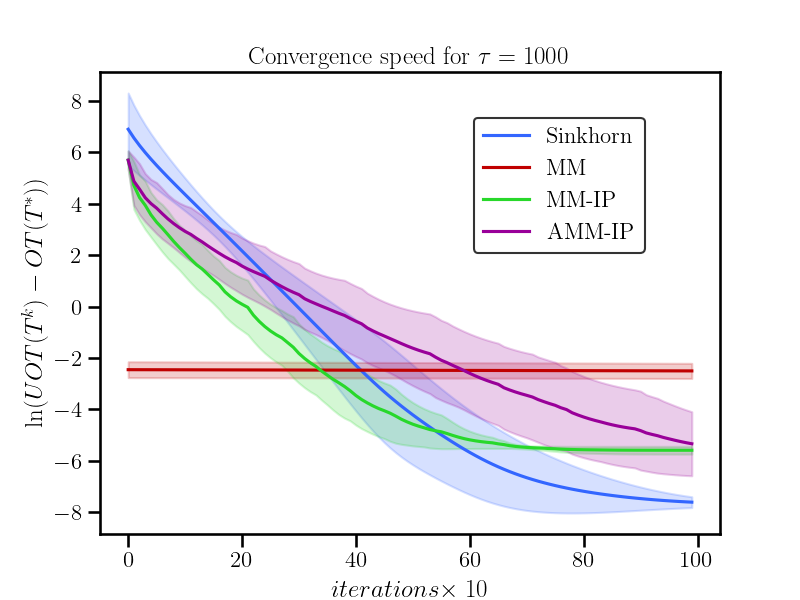
\includegraphics[width = 0.99\linewidth]{pic/ex1}
\centering
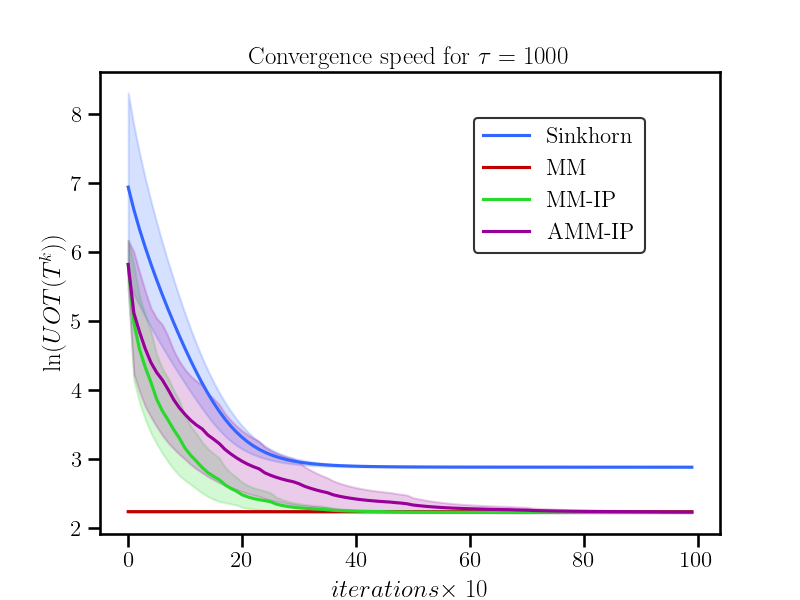
\includegraphics[width = 0.99\linewidth]{pic/ex3}
\caption{Comparison of the convergence speed for different algorithms. \changeSX{The upper plot represents the results for balanced samples, while the lower plot displays the results for unbalanced samples.} Using $\operatorname{OT}(\mat T^{*})$ to represents the value of {Eq.~(\ref{Eq:Standard_OT})}, and $\operatorname{UOT}(\mat T^{k})$ to represents the function value calculated by replacing the optimal $\mat T$ in {Eq.~(\ref{eq:uot})} with $\mat T^{k}$ }
\label{Fig:ex1}
\end{figure}



\section{Experiments}

We conducted experiments using randomly generated Gaussian distributions. In particular, we generated five pairs of 100-dimensional Gaussian distributions, each with the same mass. To test the performance of our approach in the case of unequal mass, we multiplied the mass of $\vec a$ by 1.2. For the mass-equal case, we obtained the analytical optimal solution $\mat T^{*}$ using linear programming. For both cases, we set $\tau = 1000$, and for Sinkhorn's algorithm, we set the regularizer parameter $\epsilon = 10^{-3}$. Additionally, we set the initial value of $\tilde{\tau} = 0.1$ and $q = 10^{-4}$ for our Inexact Penalized MM algorithm (MM-IP). We also incorporated Nesterov acceleration into our algorithm to obtain AMM-IP. Figure~\ref{Fig:ex1} presents the results of our experiments.


\begin{figure}[tp]
\centering
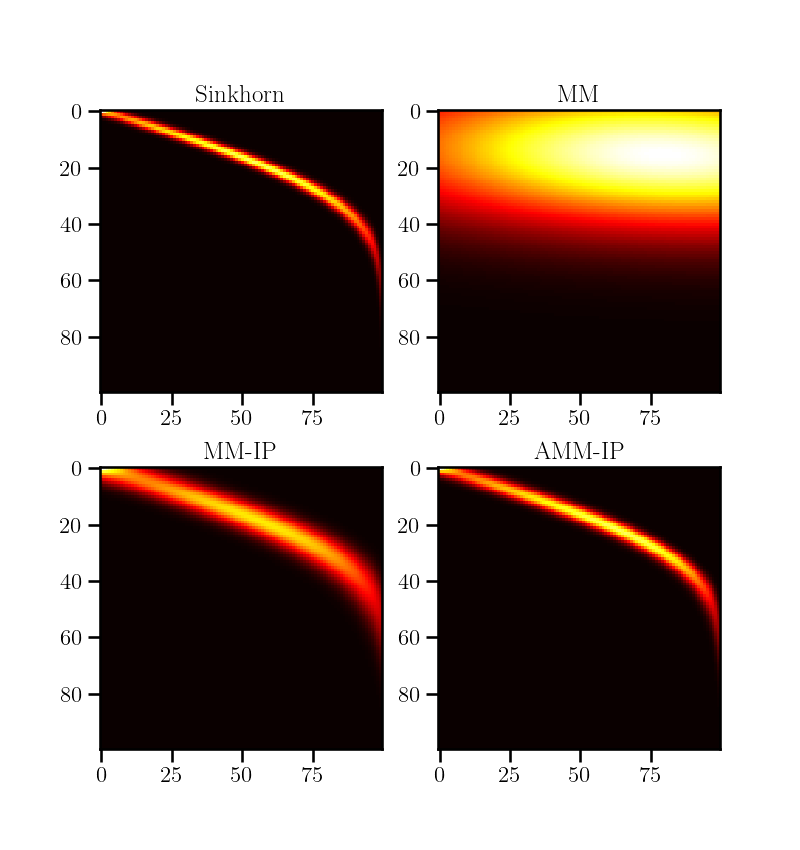
\includegraphics[width = 0.99\linewidth]{pic/ex2}
\centering
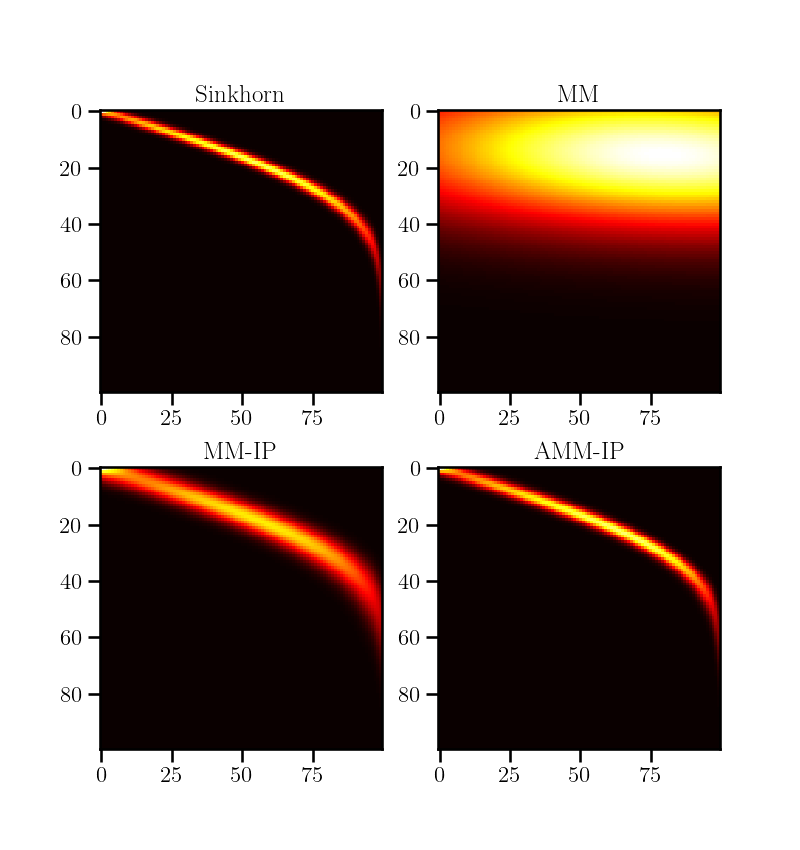
\includegraphics[width = 0.99\linewidth]{pic/ex4}
\setlength{\belowcaptionskip}{-30pt}
\caption{\changeSX{Comparison of the solutions obtained using different optimization methods over 1000 iterations, The upper plot represents the results for balanced samples, while the lower plot displays the results for unbalanced samples. The MM algorithm fails to converge quickly to a near-sparse solution in any condition. MM-IP and AMM-IP methods perform significantly better, producing solutions not only that have a similar structure to Sinkhorn's but also better accuracy for unbalanced samples.}}
\label{Fig:ex2}
\end{figure}

\changeSX{These findings indicate that the MM algorithm struggles to minimize the transport cost when faced with a large penalization parameter. This leads to a significantly higher error compared to other methods in balanced samples. In the case of unbalanced samples, the algorithm's convergence is extremely slow. This is clearly illustrated in Figure~\ref{Fig:ex2}, where the large value of $\tau$ causes the MM algorithm preserve to be dense, which is inferior to both Sinkhorn's algorithm and our proposed methods. Our approach can not only quickly produce a solution with a clear structure similar to Sinkhorn's algorithm, but also maintain a small error for unbalanced samples, where Sinkhorn suffers from errors brought by the regularizer.}



\section{Conclusion}
Our experimental results illustrate the effectiveness of our proposed Inexact Penalized MM algorithm (MM-IP). Compared to the MM algorithm, our proposed method can effectively handle the challenge of larger $\tau$ values by utilizing an inexact penalization process that avoids poor initialization. This results in a superior solution quality that is competitive with the widely-known Sinkhorn algorithm. In the future, we plan to incorporate our expertise in the field of ALM to further accelerate the MM algorithm.

\bibliographystyle{jsai}
\bibliography{ref}

%%

\end{document}

